Ogni caso d'uso può dar luogo ad una varietà di comportamenti in base alla sequenza di percorsi base ed alternativi che viene eseguita.
Per ogni caso d'uso è possibile definire un insieme di casi di test che esercitino tutti i possibili comportamenti. La dizione  ``tutti i comportamenti'' è di per sè vaga, e deve essere chiarita specificando il tipo di 
copertura (tutti gli gli archi, tutti i percorsi, etc.) che si intende usare. Comunque scelto il tipo di copertura i casi di test derivanti possono essere un numero molto elevato. Per ridurre l'ordine di grandezza di questo numero
si possono definire degli scenari di alto livello che aggreghino più casi di test insieme. In seguito si utilizza questa tecnica per effettuare un collaudo dell'applicativo.

\section{Scenari di alto livello}
Si elencano gli scenari che sono stati usato per il collaudo.

\begin{enumerate}
 \item L'Operatore inserisce una convenzione con una nuova dittà specificando una particolare ripartizione fra il personale definendo anche la prima rata. \label{MS1}
 \item L'Operatore modifica una rata di un contributo \label{MS2}
 \item L'Operatore modifica i dati di una ditta \label{MS3}
 \item L'Operatore inserisce un contributo con allegati \label{MS4}
 \item Il Docente inserisce la documentazione relativa ad una convenzione \label{MS5}
 \item L'Amministratore aggiunge un utente \label{MS6}
\end{enumerate}

In tabella \ref{macro_scenari} i casi di test esercitati per ogni scenario. Un caso di test è definito con il numero del caso d'uso corrispondente e un flusso di esecuzione (una combinazione del percorso base e di uno o più percorsi alternativi) \\


\begin{table}[h]
\label{macro_scenari}
\caption{Casi di test esercitati per scenario}
\centering
  \begin{tabular}{| c | c |} 
    \hline
    Numero di scenario & Casi di test esercitati \\
    \hline
    \ref{MS1} & \ref{UC_new_contract} base, \ref{UC_new_company} alt3, \ref{UC_new_installment}\\
    \hline
    \ref{MS2} & \ref{UC_view_contract_list} base, \ref{UC_edit_contract} base, \ref{UC_edit_installment} \\
    \hline
    \ref{MS3} & \ref{UC_view_company_list} base, \ref{UC_edit_company} base \\
    \hline
    \ref{MS4} & \ref{UC_new_contract} base\\
    \hline
    \ref{MS5} & \ref{UC_view_own_contract_list} base, \ref{UC_manage_attachments} base\\
    \hline
    \ref{MS6} & \ref{UC_new_user} base\\
    \hline
  \end{tabular} 

\end{table} 

\section{Collaudo}

\begin{itemize}
 \item Scenario \ref{MS1}\\\\
 {
 \footnotesize
  \begin{longtable}{|c|p{3cm}|p{3cm}|p{3cm}|c|}
    \hline
    Passo & Descrizione sequenza operazioni & Risultato atteso & Risultato ottenuto & Ok\\
    \hline
    1 & L'Operatore clicca sul pulsante ``Crea Convenzione'' & Viene visualizzata una schermata contenente il primo passo della procedura di creazione nel quale si possono inserire i dati generali della convenzione& Uguale 
      al risultato atteso& Sì\\
    \hline
    2 & L'Operatore clicca sul pulsante ``Aggiungi'' di fianco al campo dittà` & Viene visualizzata una finestra di dialogo contenente i dati della dittà da inserire & Uguale al risultato atteso & Sì\\
    \hline
    3 & L'Operatore inserisce i dati e clicca su ``Salva'' & Si ritorna al primo passo della procedura, la dittà appena creata è selezionata automaticamente nel menù a tendina & Uguale al risultato atteso & Sì\\
    \hline
    4 & L'Operatore clicca ``Avanti'' e passa al secondo passo della procedura, quindi inserisce una quota per il personale, infine aggiunge uno o più docenti tramite l'apposito pulsante ``Aggiungi'' in basso, in modo che la somma sia 100 & La schermata
      riflette le scelte dell'operatore aggiornando i valori percentuali dei vari campi. & Uguale al risultato atteso& Sì\\
    \hline
    5 & L'operatore clicca su ``Avanti'',quindi sul pulsante ``Aggiungi''nel passo successivo della procedura & Si apre una finestra di dialogo contenente la procedura di creazione di una rata & Uguale al risultato atteso & Sì\\
    \hline
    6  & L'Operatore inserisce i campi per la rata e completa la procedura cliccando su ``Salva'' & La finestra di dialogo si chiude e nella schermata sottostante compare la rata appena inserita & Uguale al risultato atteso & Sì\\
    \hline
    7 & L'Operatore clicca su ``Avanti'' due volte (saltando il passo relativo agli allegati) quindi clicca su``Salva'' & Si torna alla pagina iniziale & Uguale al risultato atteso & Sì \\
    \hline
    8 & L'Operatore clicca su ``Visualizza elenco contratti'' & Si apre un elenco di contratti fra cui è possibile ritrovare la convenzione appena inserita & Uguale al risultato atteso & Sì\\
    \hline
\end{longtable}
}

 \item Scenario \ref{MS2}\\\\
 {
 \footnotesize
  \begin{longtable}{|c|p{3cm}|p{3cm}|p{3cm}|c|}
    \hline
    Passo & Descrizione sequenza operazioni & Risultato atteso & Risultato ottenuto & Ok\\
    \hline
    1 & L'Operatore clicca sul pulsante ``Visualizza lista contratti'' & Viene visualizzata una schermata contenente l'elenco dei contratti & Uguale 
      al risultato atteso& Sì\\
    \hline
    2 & L'Operatore seleziona la convenzione di cui si vuole modificare la rata, quindi clicca sul pulsante ``Modifica'' che appare a destra sulla riga selezionata& Viene visualizzata una schermata divisa in schede che mostra i dettagli
    della convenzione& Uguale al risultato atteso & Sì\\
    \hline
    3 & L'Operatore raggiunge la scheda ``Rate'' quindi dopo avere selezionato la rata desiderata dall'elenco clicca sul pulsante ``Modifica'' che appare sulla sinistra& Appare una finestra di dialogo che mostra i dettagli della rata & Uguale al risultato atteso & Sì\\
    \hline
    4 & L'Operatore effettua le modifiche desiderate e clicca su ``Salva'' & La finestra di dialogo si chiude e riappare la schermata sottostante & Uguale al risultato atteso& Sì\\
    \hline
    5 & L'operatore clicca su ``Salva''& Si torna all'elenco delle convenzioni & Uguale al risultato atteso & Sì\\
    \hline
    6  & L'Operatore ripetendo il procedimento appena compiuto riapre (in lettura) la rata appena modificata & Si apre una finestra di dialogo che contiene i dati della rata appena modificati & Uguale al risultato atteso & Sì\\
    \hline
\end{longtable}
}


 \item Scenario \ref{MS3}\\\\
 {
 \footnotesize
  \begin{longtable}{|c|p{3cm}|p{3cm}|p{3cm}|c|}
    \hline
    Passo & Descrizione sequenza operazioni & Risultato atteso & Risultato ottenuto & Ok\\
    \hline
    1 & L'Operatore clicca sul pulsante ``Visualizza lista ditte'' & Viene visualizzata una schermata contenente l'elenco delle ditte & Uguale 
      al risultato atteso& Sì\\
    \hline
    2 & L'Operatore seleziona la ditta da modificare, quindi clicca sul pulsnate ``Modifica'' che appare a sinistra sulla riga selezionata& Viene visualizzata una finestra di dialogo che mostra i dettagli
    della ditta& Uguale al risultato atteso & Sì\\
    \hline
    3 & L'Operatore effettua le modifiche desiderate e clicca su ``Salva''& La finestra di dialogo si chiude e riappare l'elenco delle ditte & Uguale al risultato atteso & Sì\\
    \hline
    4 & L'Operatore seleziona la ditta appena modificata e clicca sul ``Visualizza'' & Si apre una finestra di dialogo contente i dati della ditta appena modificata & Uguale al risultato atteso& Sì\\
    \hline
\end{longtable}
}

 \item Scenario \ref{MS4}\\\\
 {
 \footnotesize
  \begin{longtable}{|c|p{3cm}|p{3cm}|p{3cm}|c|}
    \hline
    Passo & Descrizione sequenza operazioni & Risultato atteso & Risultato ottenuto & Ok\\
    \hline
    1 & L'Operatore clicca sul pulsante ``Crea contributo'' & Viene visualizzata una schermata contenente il primo passo della procedura di creazione nel quale si possono inserire i dati generali del contributo& Uguale 
      al risultato atteso& Sì\\
    \hline
    2 & L'Operatore riempie i dati generali del contributo, quindi clicca su ``Avanti'' due volte saltando la scheda relativa alle rate & Viene visualizzata la scheda ``Allegati'' & Uguale al risultato atteso & Sì \\
    \hline
     3 & L'Operatore clicca su ``Aggiungi''& Compare una finestra di dialogo che permettere si sciegliere un file da allegare & Uguale al risultato atteso & Sì \\
    \hline
    4 & L'Operatore seleziona un file tramite la finestra di dialogo & La finestra di dialogo si chiude e il file scelto appare nella lista degli allegati caricati & Uguale al risultato atteso & Sì\\
    \hline
    5 & L'Operatore clicca ``Avanti'' quindi su ``Salva'' & Riappare la schermata inziale & Uguale al risultato atteso & Sì\\
    \hline
    6 & L'Operatore clicca su ``Visualizza contratti''& Si apre la lista dei contratti che ora contiene anche il contributo appena inserito & Uguale al risultato atteso & Sì\\    
    \hline
\end{longtable}

}


 \item Scenario \ref{MS5}\\\\
 {
 \footnotesize
  \begin{longtable}{|c|p{3cm}|p{3cm}|p{3cm}|c|}
    \hline
    Passo & Descrizione sequenza operazioni & Risultato atteso & Risultato ottenuto & Ok\\
    \hline
    1 & Il Docente clicca sul pulsante ``Visualizza lista contratti'' & Viene visualizzata una schermata contenente la lista dei contratti di cui il docente è responsabile scientifico& Uguale 
      al risultato atteso& Sì\\
    \hline
    2 &Il Docente seleziona la convenzione a cui è interessato, quindi clicca sul pulsante ``Visualizza'' che compare sulla sinistra& Viene visualizzata una schermata suddivisa in schede contenente i dati della convenzione & Uguale al risultato atteso & Sì \\
    \hline
     3 & Il Docente raggiunge la scheda ``Allegati'' quindi clicca ``Aggiungi'''& Compare una finestra di dialogo che permettere si sciegliere un file da allegare & Uguale al risultato atteso & Sì \\
    \hline
    4 & Il Docente seleziona un file tramite la finestra di dialogo & La finestra di dialogo si chiude e il file scelto appare nella lista degli allegati caricati & Uguale al risultato atteso & Sì\\
    \hline
    5 & Il Docente clicca su``Salva'' & Riappare la lista dei contratti & Uguale al risultato atteso & Sì\\
    \hline
    6 & Il Docente ripete la procedura fino ad aprire la scheda ``Allegati'' & La scheda allegati contiene i file appena inseriti & Uguale al risultato atteso & Sì\\    
    \hline
\end{longtable}

}


 \item Scenario \ref{MS6}\\\\
 {
 \footnotesize
  \begin{longtable}{|c|p{3cm}|p{3cm}|p{3cm}|c|}
    \hline
    Passo & Descrizione sequenza operazioni & Risultato atteso & Risultato ottenuto & Ok\\
    \hline
    1 & L'Amministratore clicca sul pulsante ``Aggiungi utente'' & Viene visualizzata una schermata contenente contenente i campi da inserire per il nuovo utente& Uguale 
      al risultato atteso& Sì\\
    \hline
    2 & L'Amministratore riempi i campi quindi clicca su ``Salva''& Si torna alla pagina iniziale & Uguale al risultato atteso & Sì \\
    \hline
     3 & L'Amministratore clicca su ``Visualizza lista utenti''& Compare una lista contente tutti gli utenti, fra i quali anche quello appena inserito & Uguale al risultato atteso & Sì \\
    \hline
\end{longtable}

}
\end{itemize}

\begin{figure}
	\centering
	\scalebox{0.5}{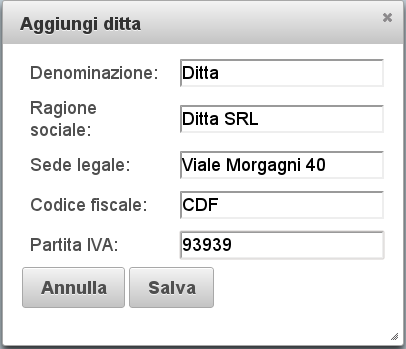
\includegraphics{Aggiungi_Ditta_Dialog.png}}
	\caption{Inserimento Ditta - Scenario 1 Passo 2}
	\label{aggiungiDitta}
\end{figure}

\begin{figure}
	\centering
	\scalebox{0.25}{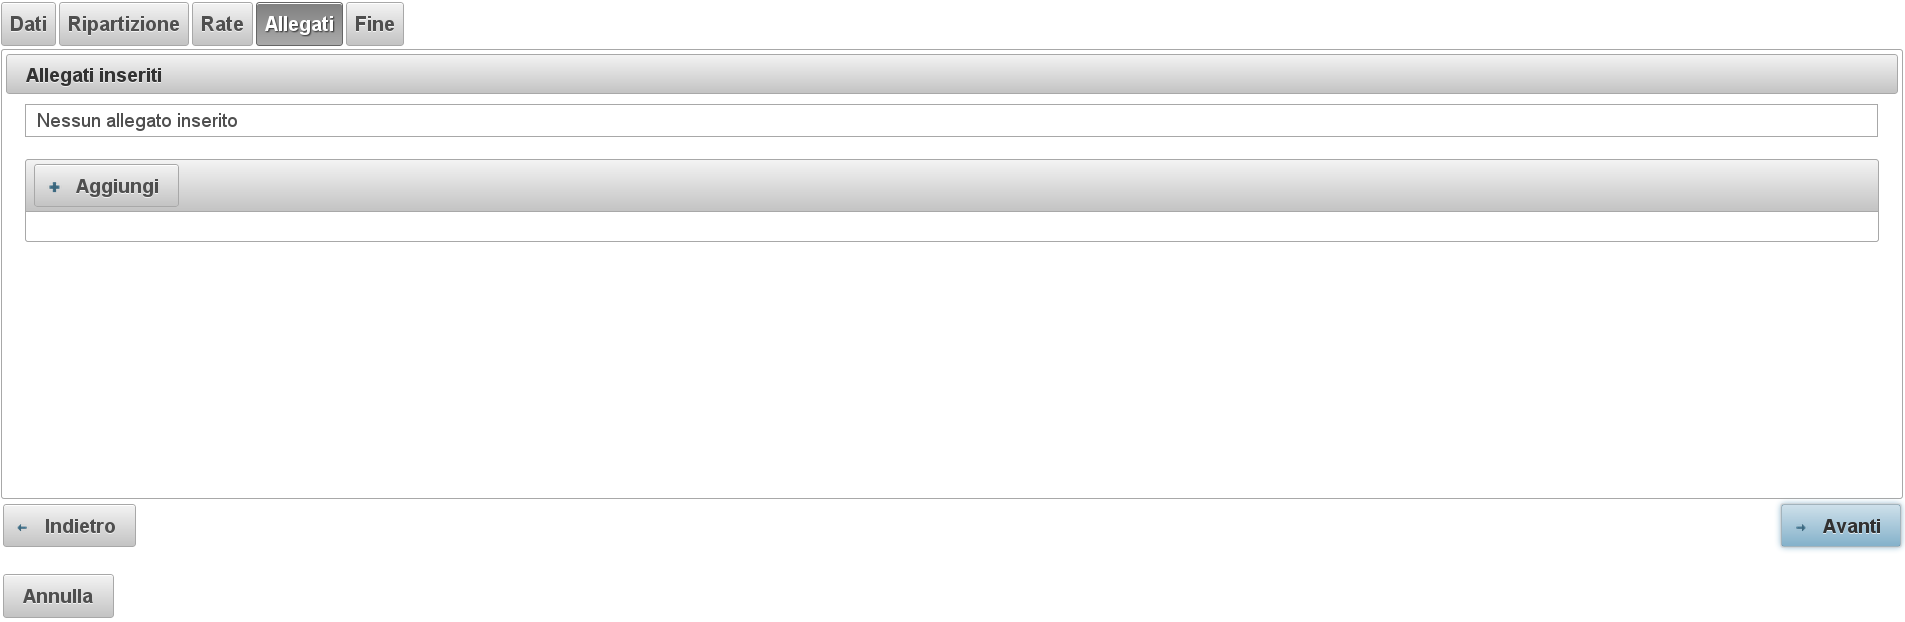
\includegraphics{Allegati.png}}
	\caption{Lista Allegati - Scenario 4 Passo 2}
	\label{allegati}
\end{figure}

\begin{figure}
	\centering
	\scalebox{0.25}{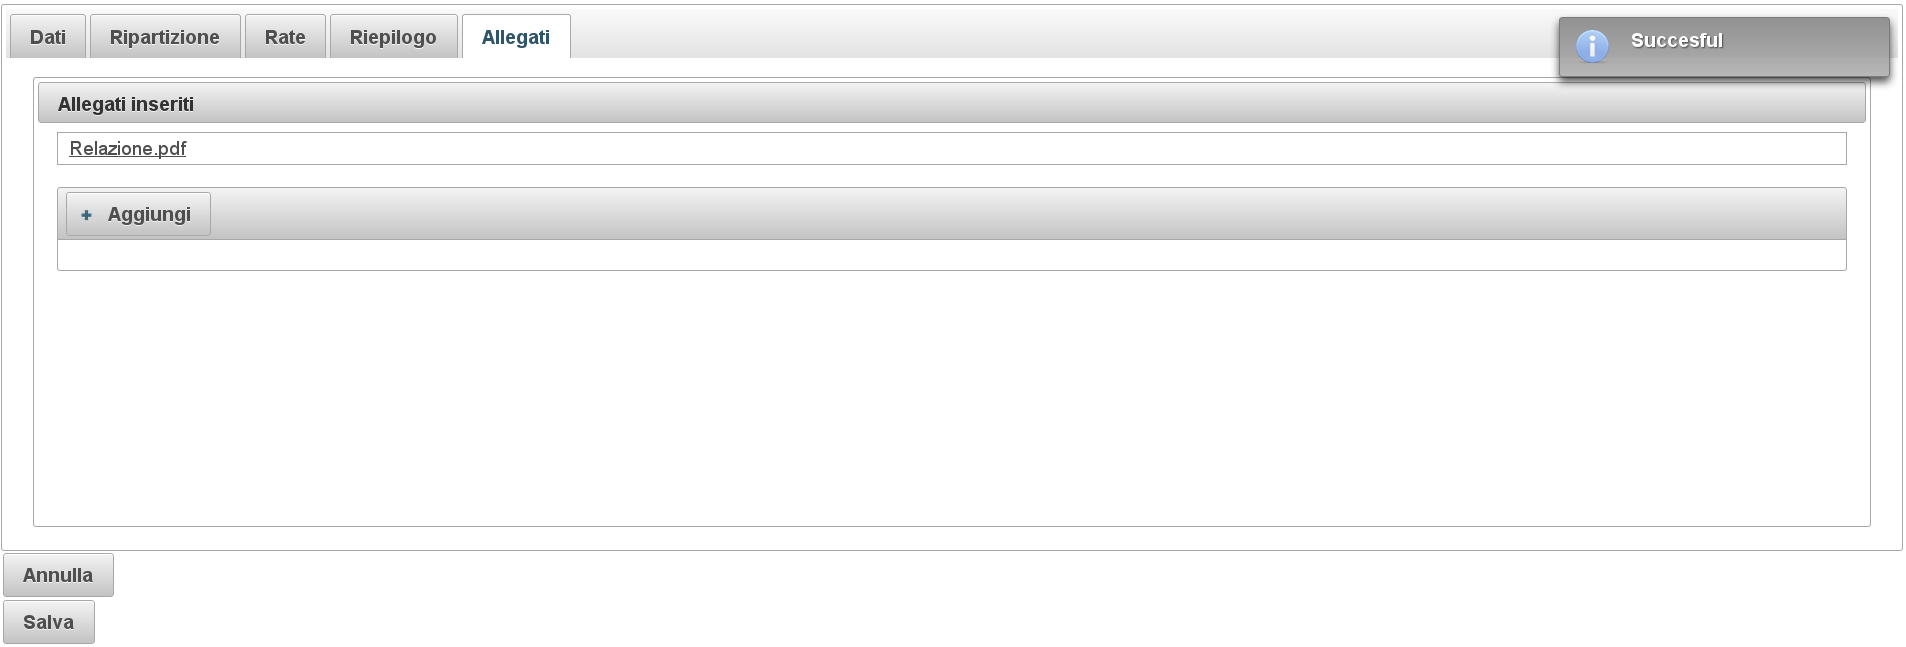
\includegraphics{Allegato_Inserito.png}}
	\caption{Inserimento Allegato - Scenario 5 Passo 5}
	\label{allegatiDopoInserimento}
\end{figure}

\begin{figure}
	\centering
	\scalebox{0.25}{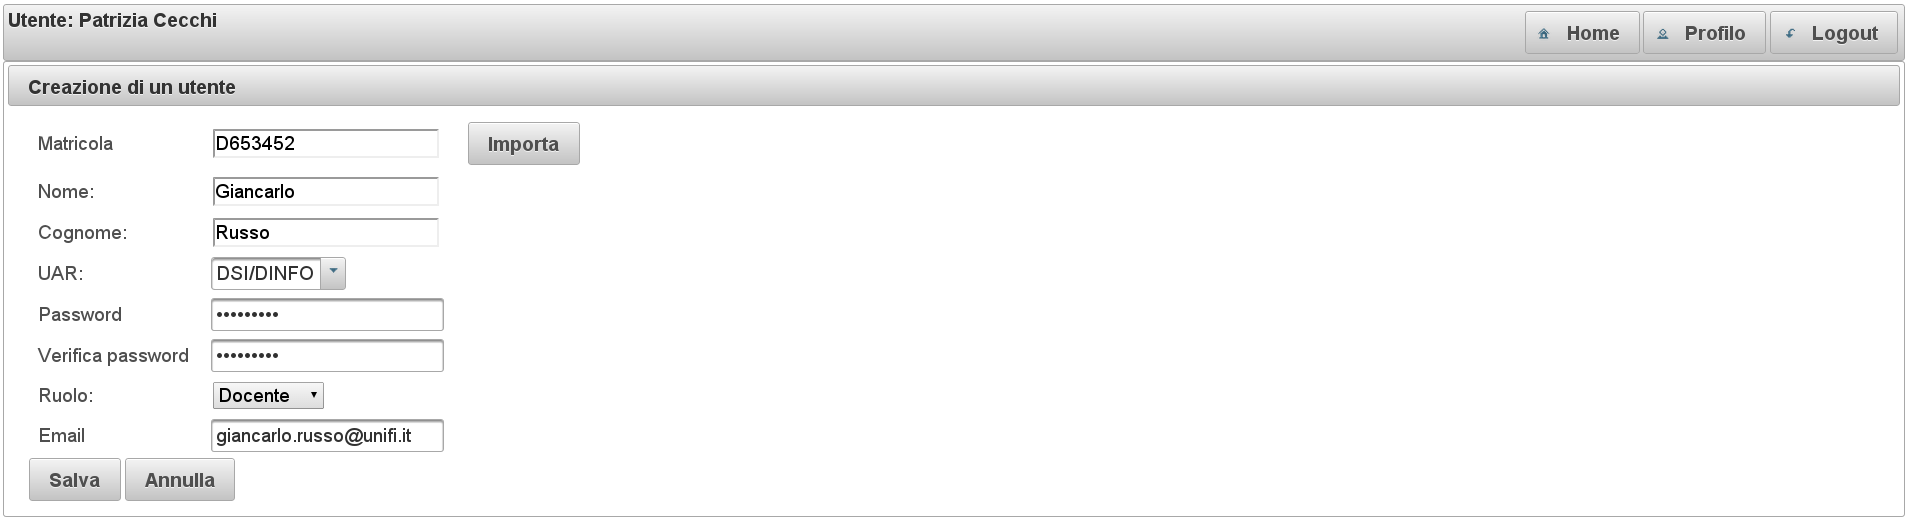
\includegraphics{Creazione_Utente.png}}
	\caption{Inserimento utente - Scenario 6 Passo 2}
	\label{creazioneUtente}
\end{figure}

\begin{figure}
	\centering
	\scalebox{0.3}{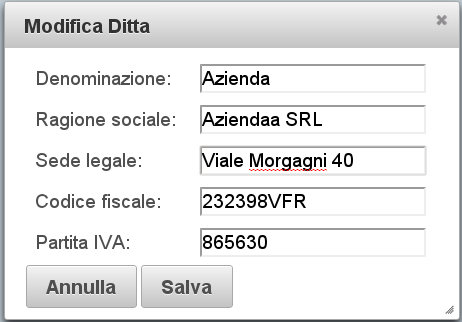
\includegraphics{Dialog_Ditta_Modifica.png}}
	\caption{Modifica Ditta - Scenario 3 Passo 3}
	\label{modificaDitta}
\end{figure}

\begin{figure}
	\centering
	\scalebox{0.25}{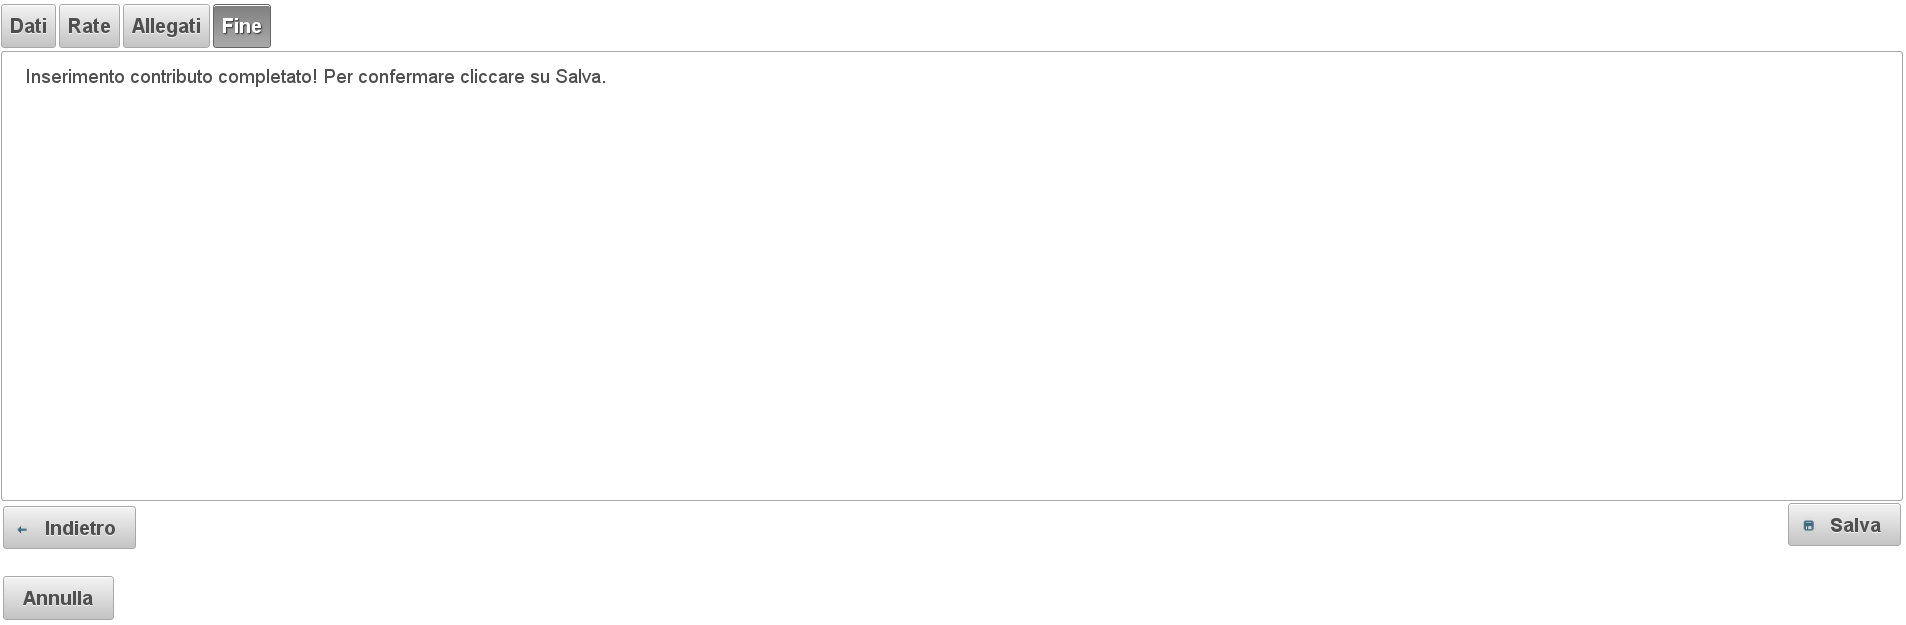
\includegraphics{Fine_Contributo.png}}
	\caption{Salvataggio contributo - Scenario 4 Passo 5}
	\label{fineContributo}
\end{figure}

\begin{figure}
	\centering
	\scalebox{0.25}{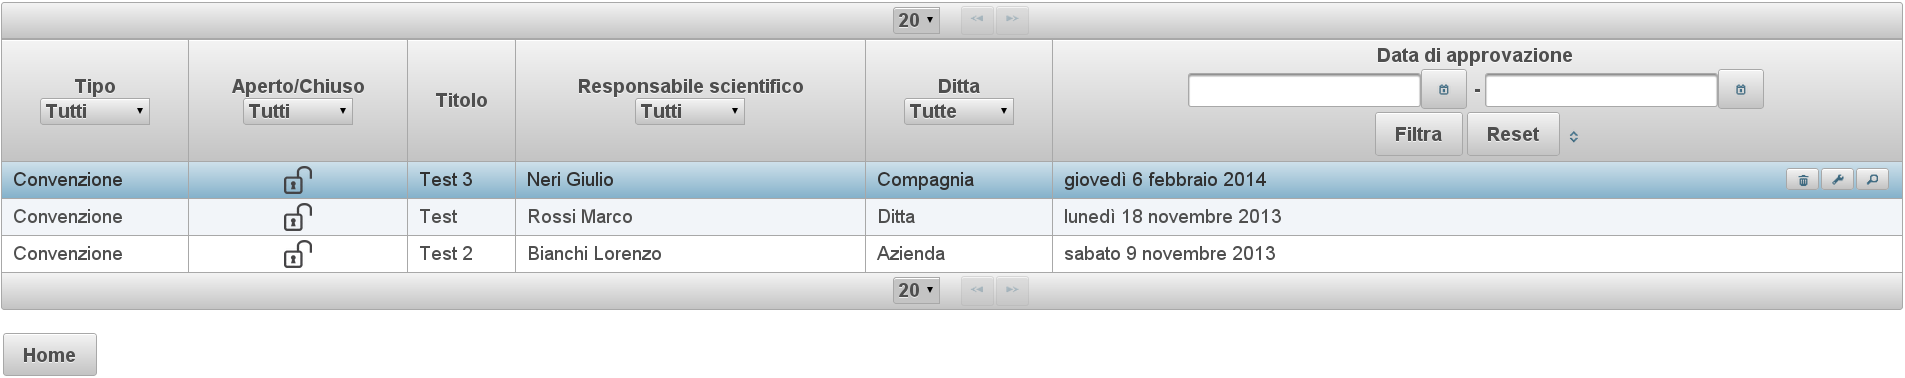
\includegraphics{Lista_Convenzioni.png}}
	\caption{Lista Contratti - Scenario 2 Passo 2}
	\label{Lista delle convenzioni/contributi}
\end{figure}

\begin{figure}
	\centering
	\scalebox{0.25}{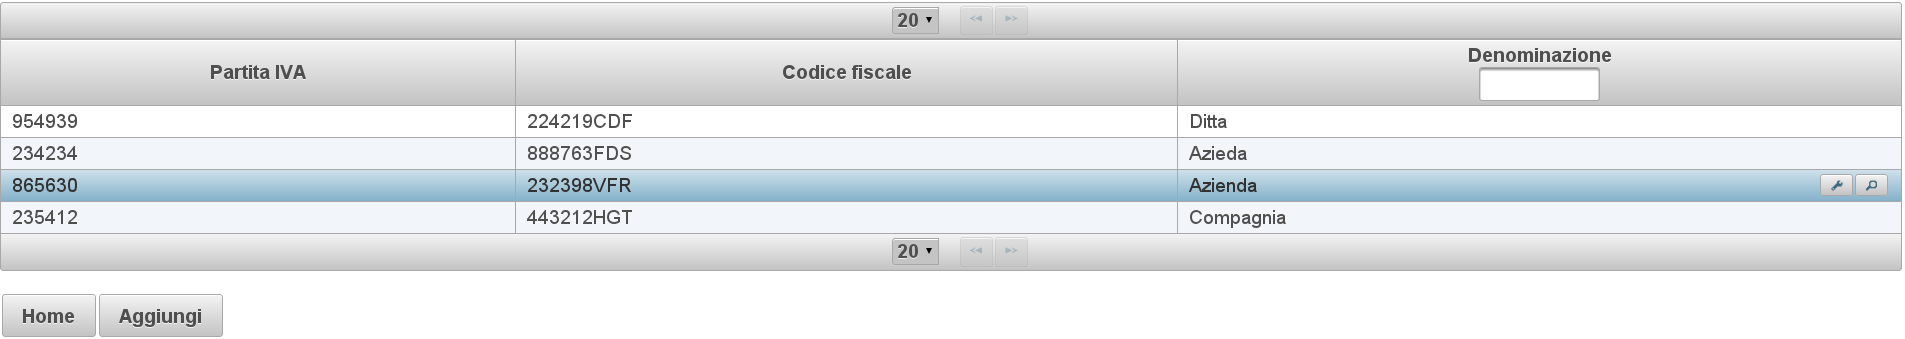
\includegraphics{Lista_ditte_modifica.png}}
	\caption{Lista ditte - Scenario 3 Passo 2}
	\label{ListaDitte}
\end{figure}

\begin{figure}
	\centering
	\scalebox{0.25}{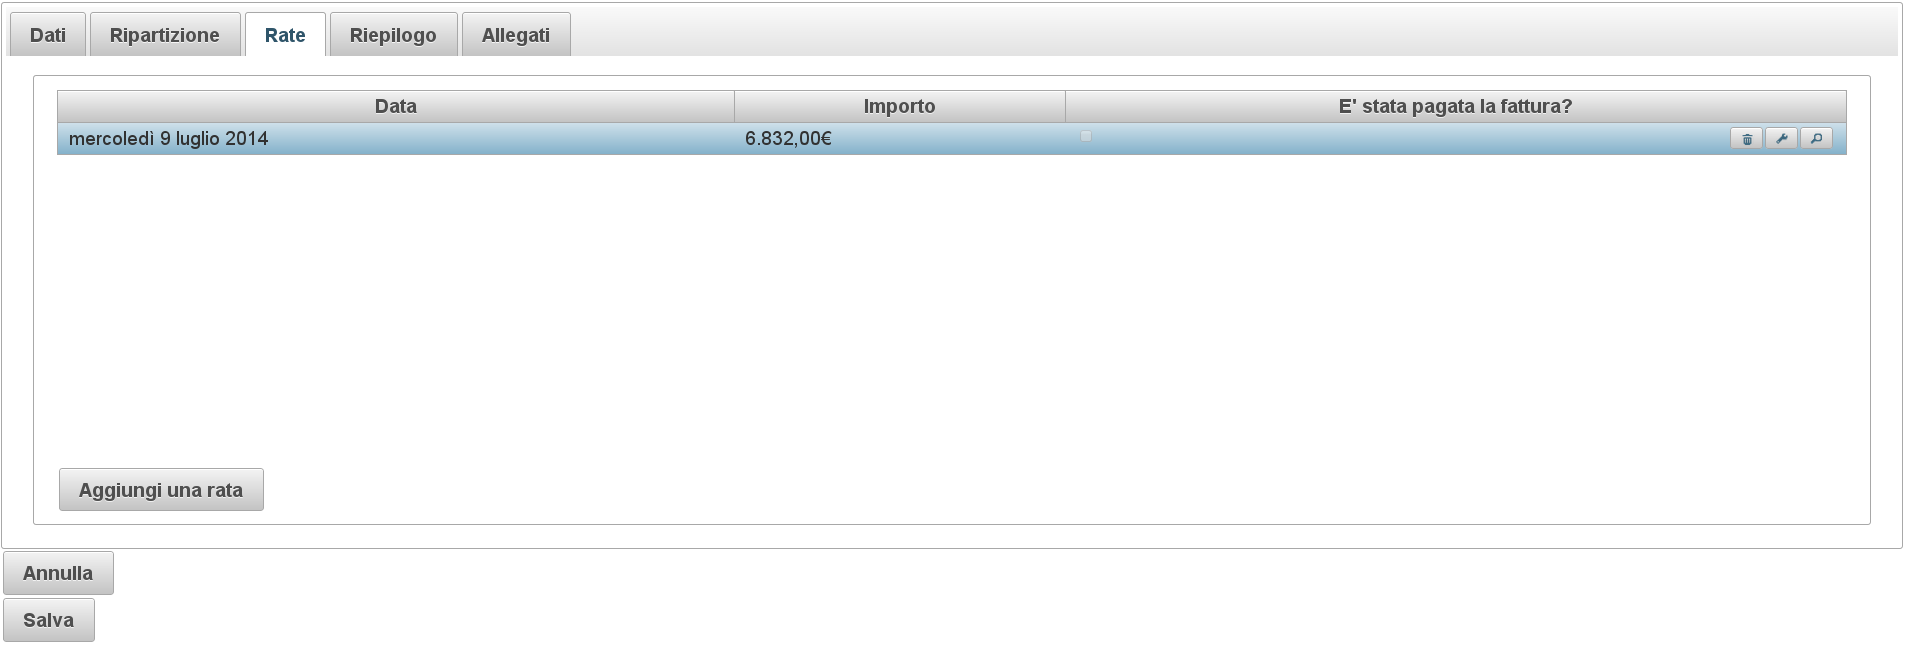
\includegraphics{Lista_Rate_Modifica.png}}
	\caption{Lista rate - Scenario 2 Passo 3}
	\label{ListaRate}
\end{figure}

\begin{figure}
	\centering
	\scalebox{0.25}{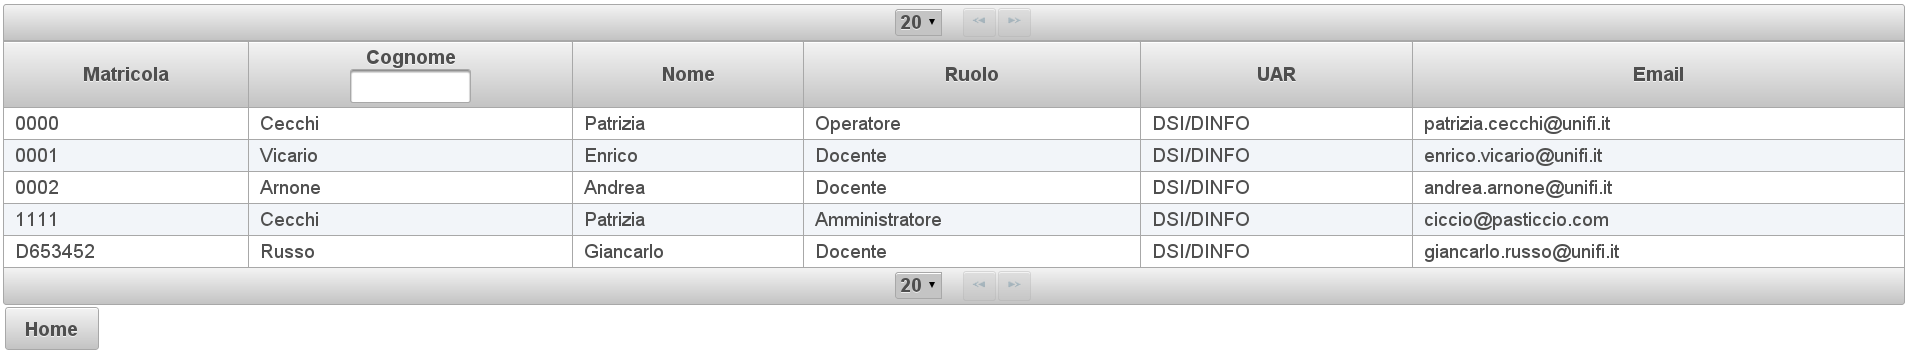
\includegraphics{Lista_utenti.png}}
	\caption{Lista utenti - Scenario 6 Passo 3}
	\label{ListaUtenti}
\end{figure}

\begin{figure}
	\centering
	\scalebox{0.28}{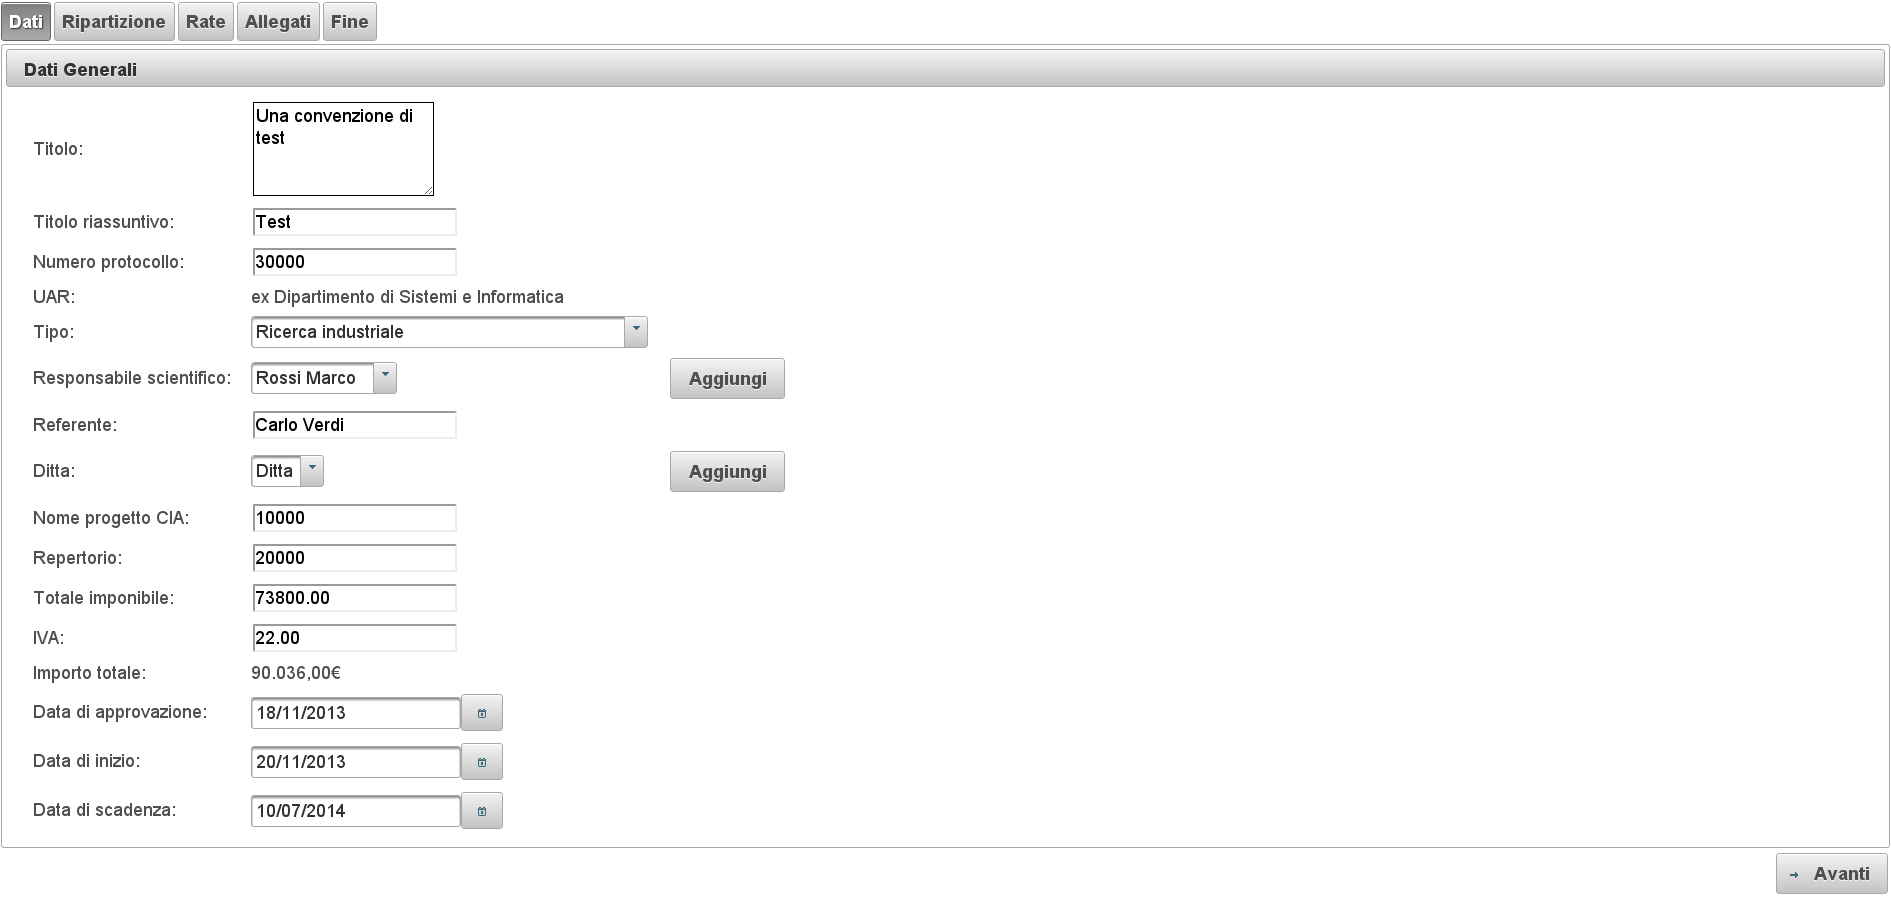
\includegraphics{Tab_Dati.png}}
	\caption{Dati convenzione - Scenario 1 Passo 1}
	\label{tabDati}
\end{figure}

\begin{figure}
	\centering
	\scalebox{0.28}{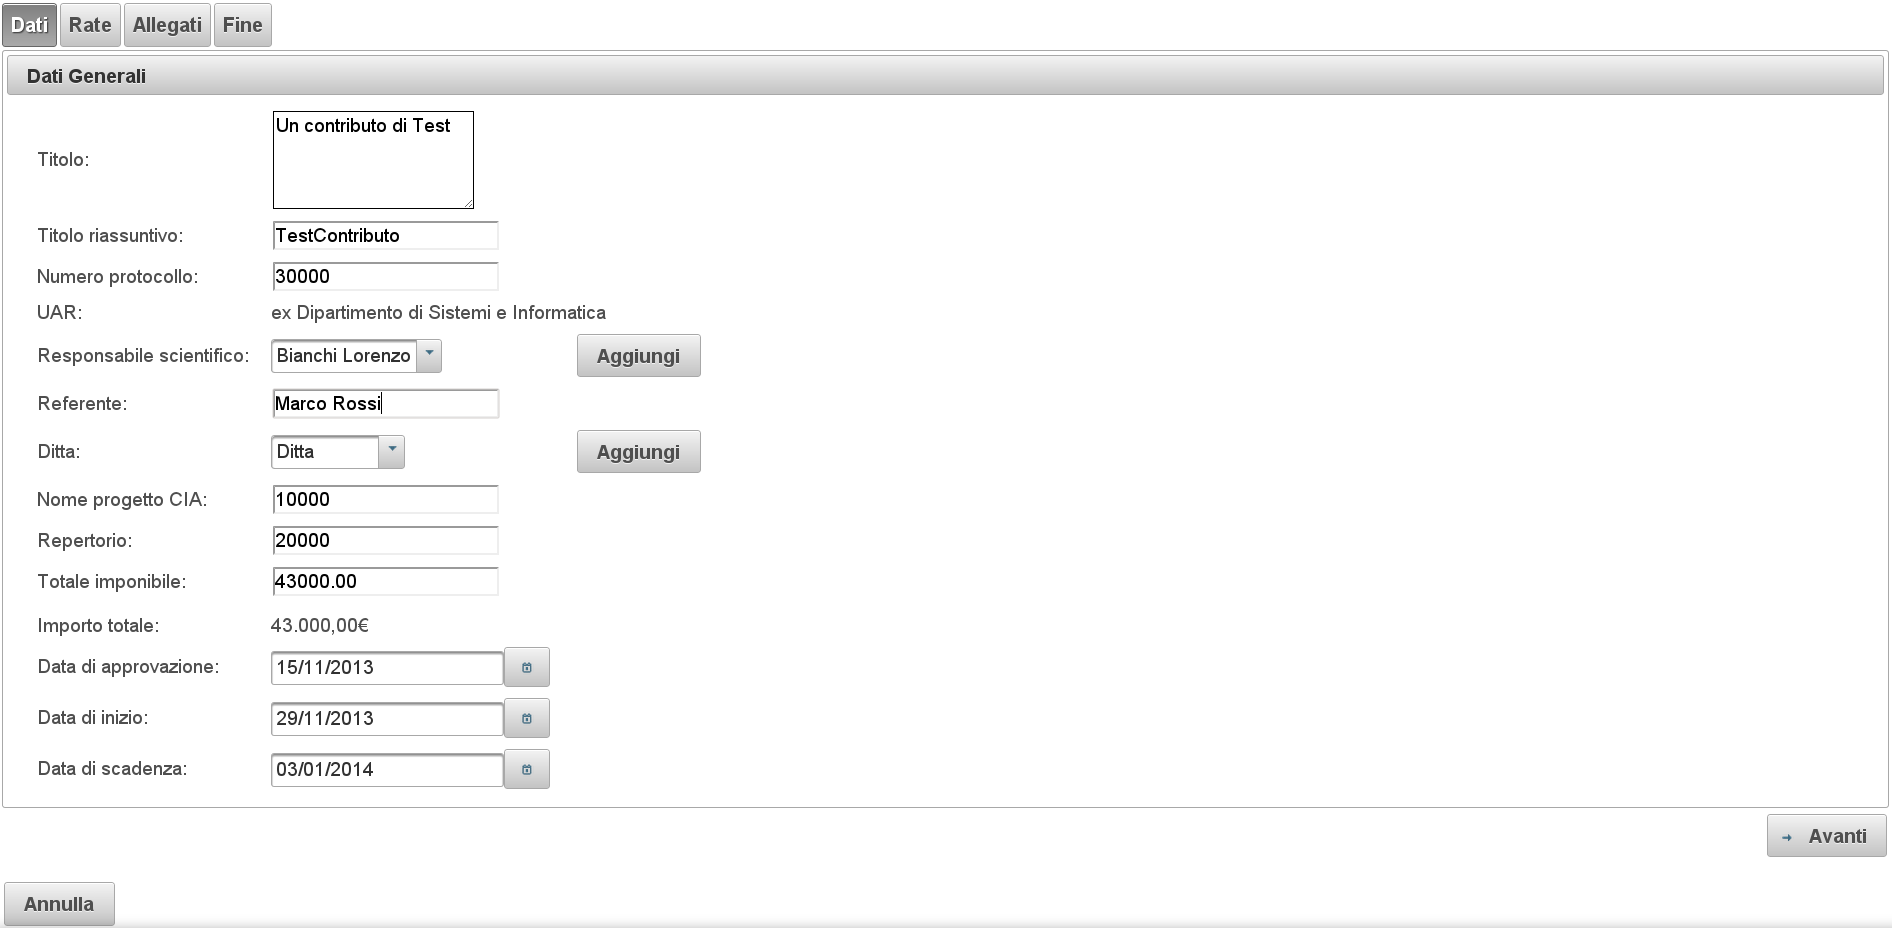
\includegraphics{Tab_Dati_Contributo.png}}
	\caption{Dati Contributo - Scenario 4 Passo 1}
	\label{tabDatiContributo}
\end{figure}

\begin{figure}
	\centering
	\scalebox{0.28}{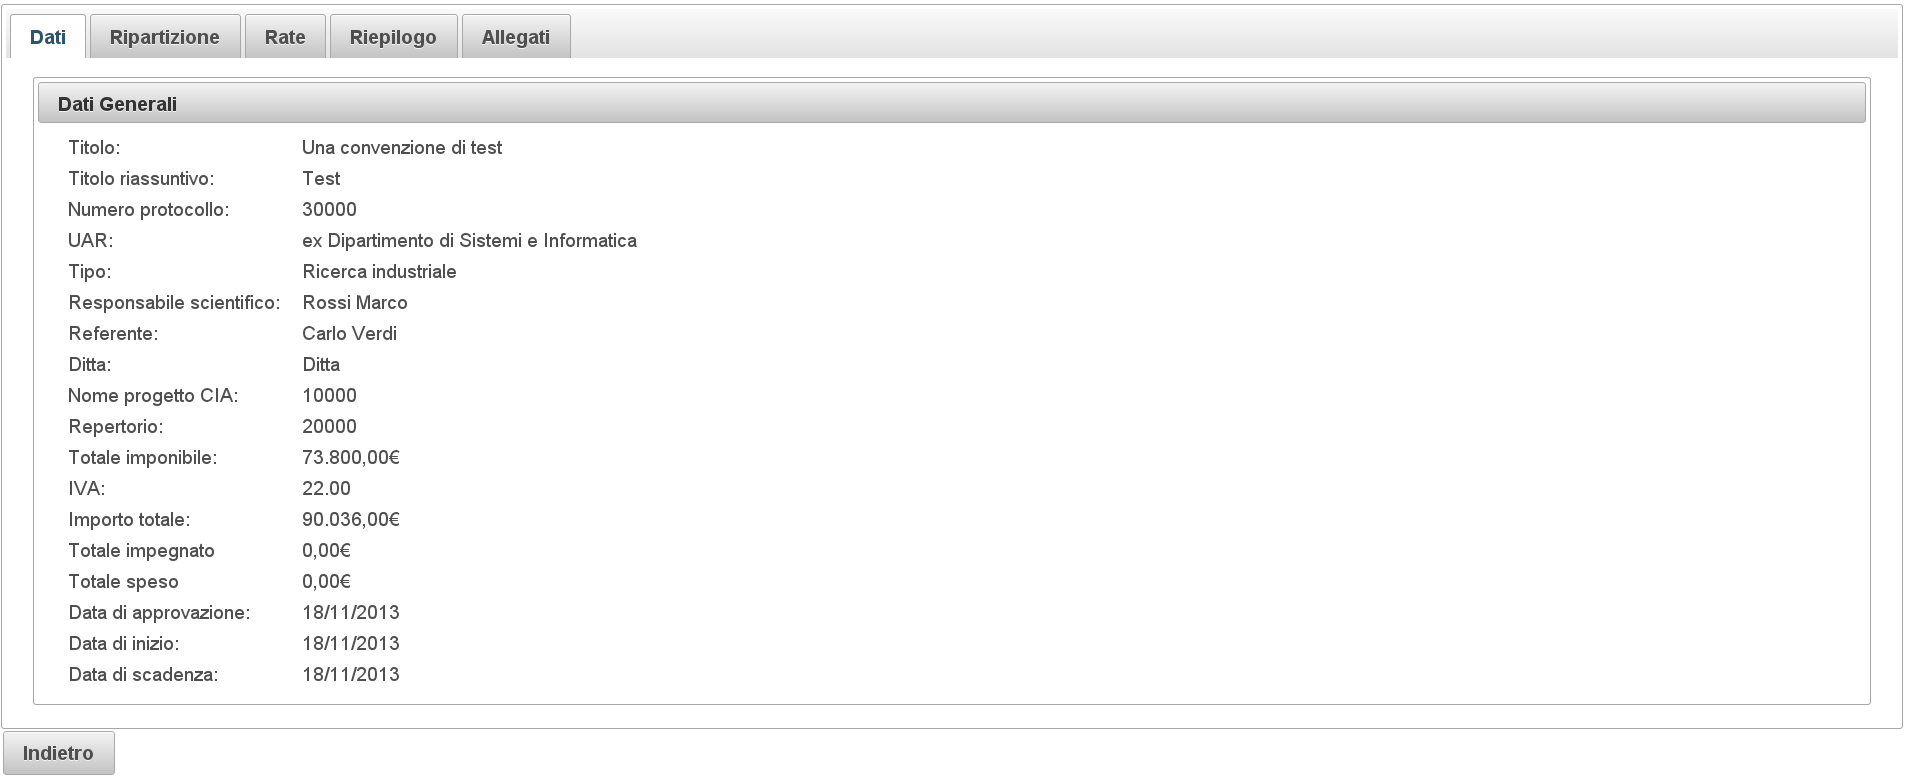
\includegraphics{Tab_Dati_visualizzazione.png}}
	\caption{Visualizzazione convenzione - Scenario 5 Passo 1}
	\label{tabDatiVisualizzazione}
\end{figure}

\begin{figure}
	\centering
	\scalebox{0.28}{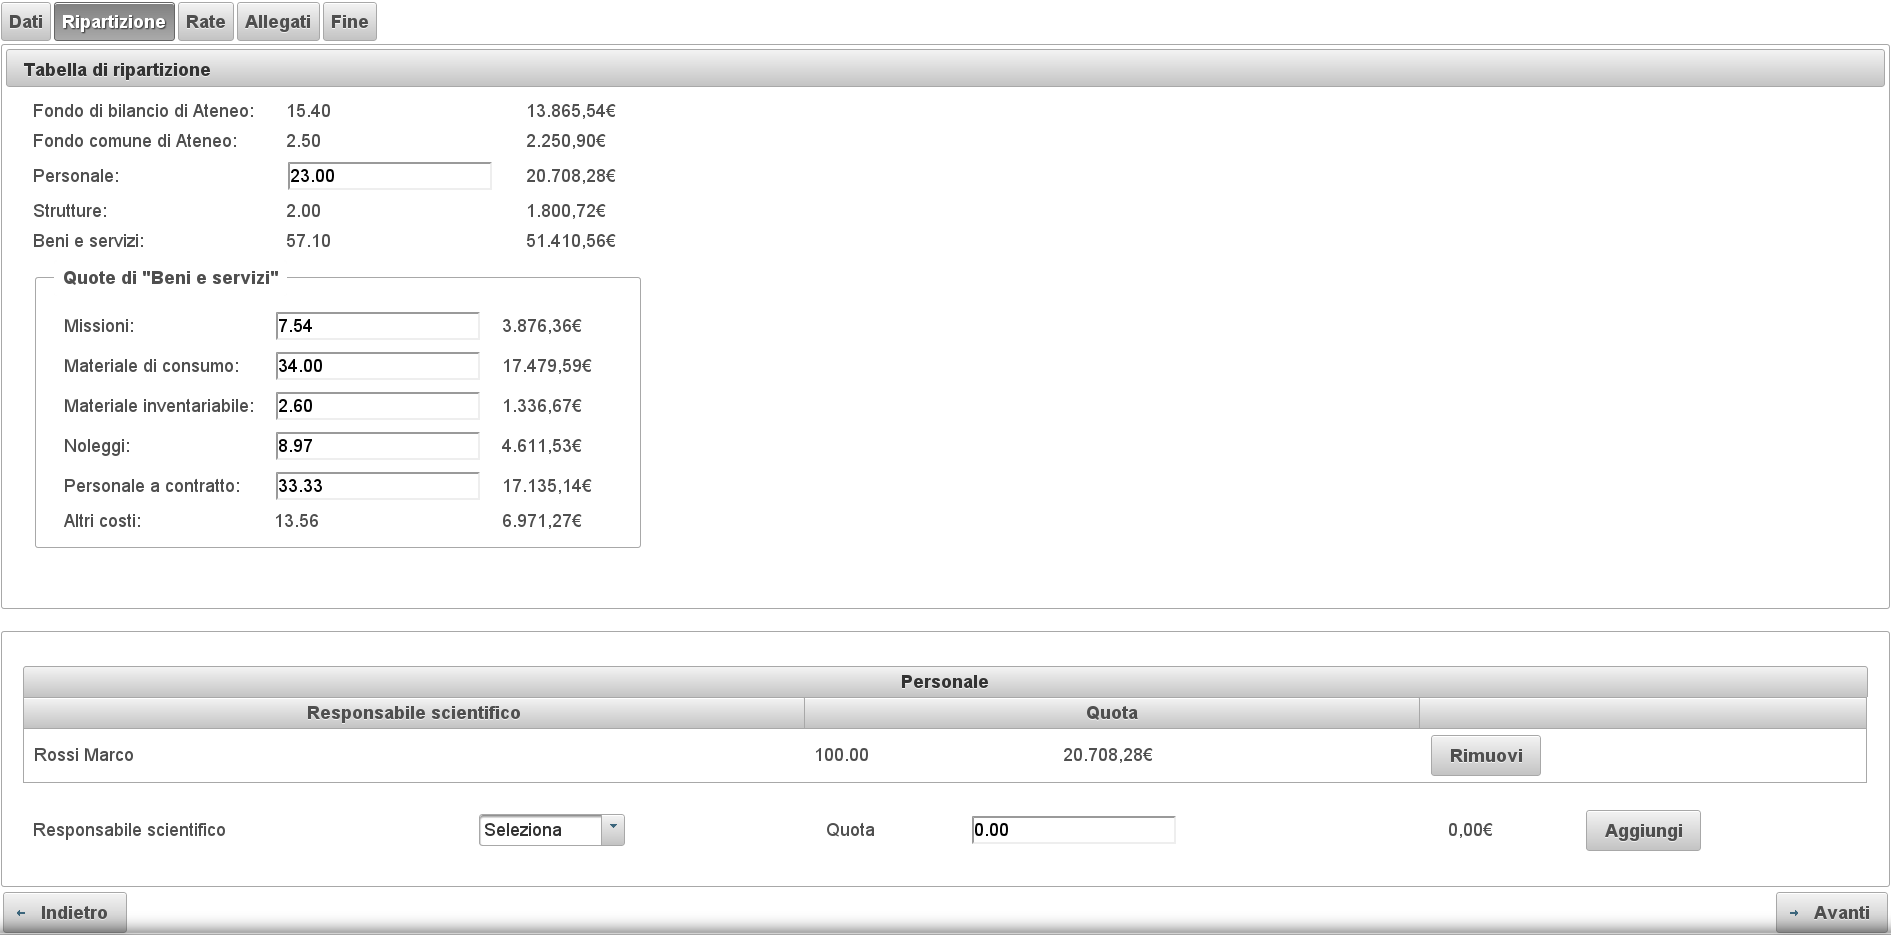
\includegraphics{Tab_Rip.png}}
	\caption{Tabella Ripartizione - Scenario 1 Passo 4}
	\label{tabRip}
\end{figure}

\begin{figure}
	\centering
	\scalebox{0.28}{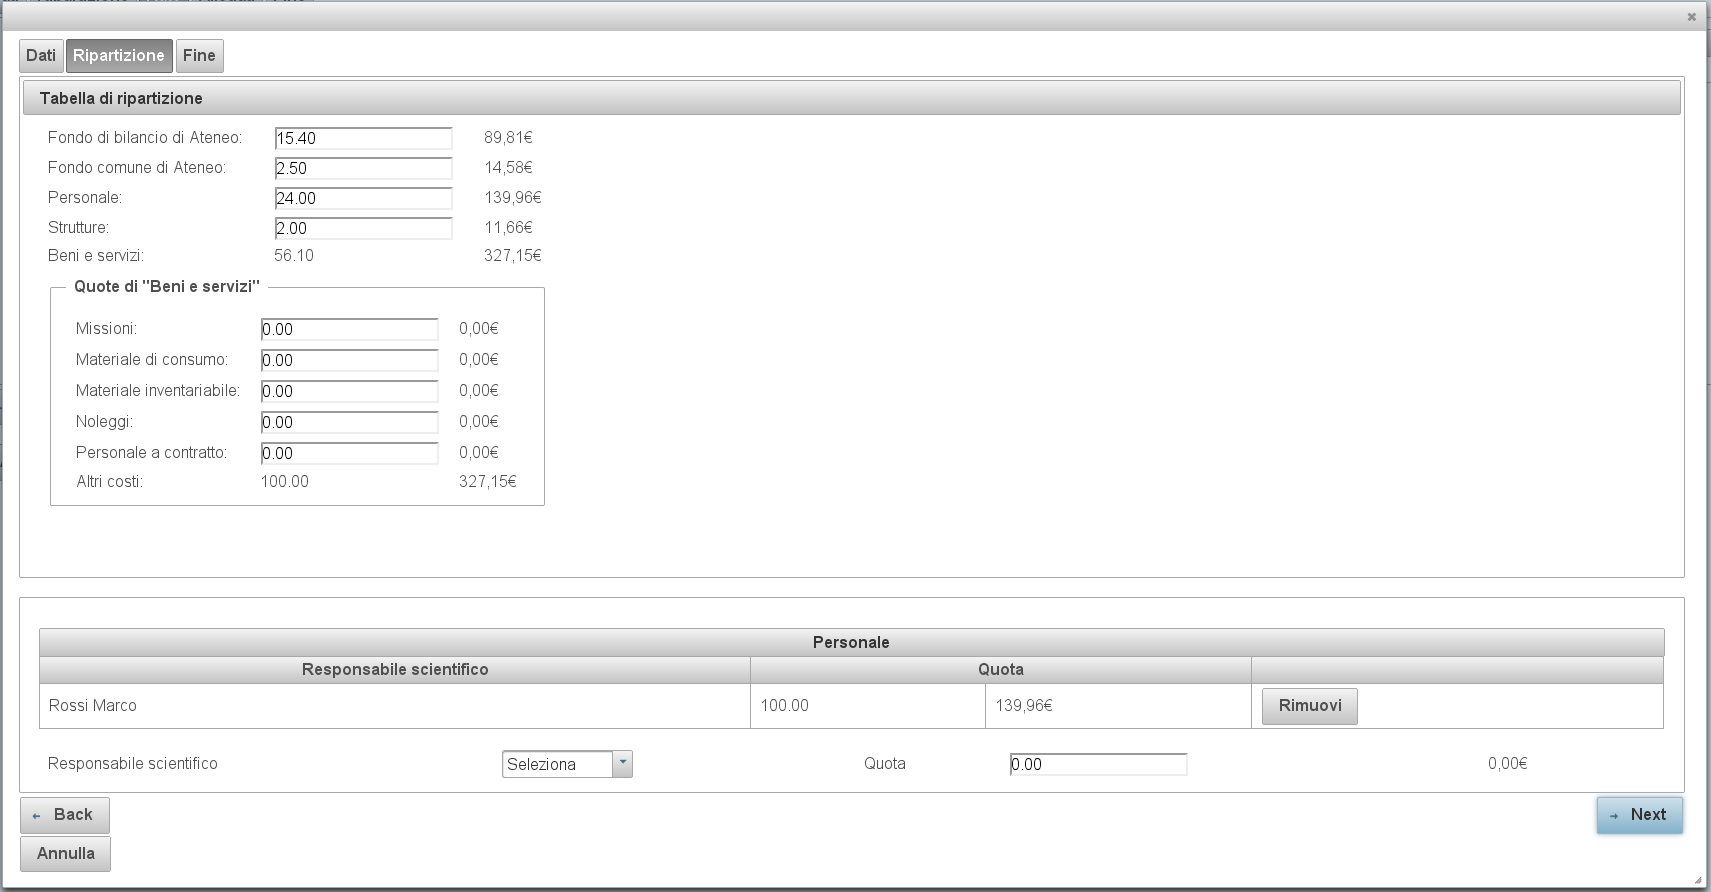
\includegraphics{Tab_Rip_Rata.png}}
	\caption{Tabella Ripartizione Rata - Scenario 1 Passo 6}
	\label{tabRipRata}
\end{figure}